\documentclass[twocolumn]{article}
\usepackage[a4paper, top=1in, bottom=1in, left=2cm, right=2cm]{geometry}
\usepackage[singlespacing]{setspace}
\usepackage{amsmath}
\usepackage{amssymb}
\usepackage{graphicx}
\usepackage{hyperref}
\title{Rediscovery of astroid from the refraction image by a flat boundary}
\author{M. Ryu \\ {\href{mailto:mingshey@hafs.hs.kr}{mingshey@hafs.hs.kr}}}
\begin{document}
\maketitle
\section{Introduction}
If you see a point object under water from  above the flat surface of water, 
the position of image depends on the point of view(POV). The image seen
 within a normal plane traces out a specific curve that is called a  
 \emph{squashed astroid} as the POV moves around.

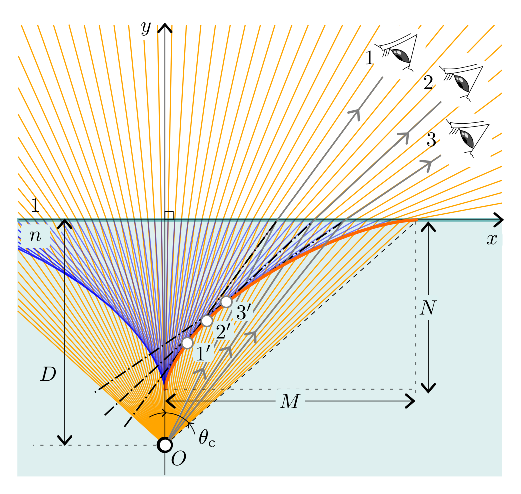
\includegraphics[width=2.7in]{g409.eps}

Let the normal plane that contains the object and  POV be the $xy$-plane,
 and let the intersection of  normal plane and the surface of water be the 
 $x$-axis, and the normal through  object $y$-axis. Then the trace of image 
 is part of the curve 
$$ \left| \dfrac{x}{M} \right| ^ {2/3} 
+ \left| \dfrac{y}{N} \right| ^ {2/3} = 1,$$
where $M = D/\sqrt{n^2 - 1}$ is the maximum distance of incidence
determined by the critical angle of total internal reflection and $N = D/n$ 
is the apparent depth of the object when observed from directly above, where
$D$ is the actual depth of the object, and $n$ is the refractive index of 
water relative to the air.

\section{Derivation of the formula}
Let the refractive indices  of air and water be $n_1$ and $n_2$, respectively. 
The point object $O$ is at the depth $D$ below the boundary of air and water. 
A ray starts off the object and enters the boundary of media at $\alpha$ away 
from the $y$-axis with angle $\theta_2$ from the normal at that point and then 
refracts into air with angle $\theta_1$ from the same normal.

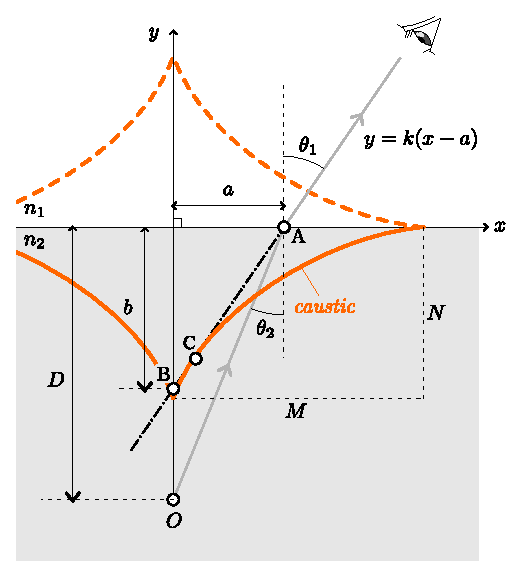
\includegraphics[width=2.2in]{g237.eps}

From Snell's law we have
$$ \sin\theta_1 = \frac{n_2}{n_1} \sin\theta_2 = n\sin\theta_2.$$
The extension of refracted ray is described by the equation 
$$y=k(x-\alpha),$$
where 
$$k=\dfrac{1}{\tan\theta_1}=\dfrac{\cos\theta_1}{\sin\theta_1},$$
and considering the Snell's law,
$$k=\dfrac{\sqrt{1-n^2\sin^2\theta_2}}{n\sin\theta_2}.$$
This line meets the $y$-axis at $y=\beta$, thus
$$\beta = -k\alpha.$$
By the geometry we have
$$\alpha = D\tan\theta_2 = \dfrac{D\sin\theta_2}{\cos\theta_2},$$
and
$$\begin{aligned}
	\beta &= -k\alpha \\
	&= -\dfrac{D\sin\theta_2}{\cos\theta_2}
	\dfrac{\sqrt{1-n^2\sin\theta_2}}{n\sin\theta_2}\\
	&=-\dfrac{D\sqrt{1-n^2\sin\theta_2}}{n\cos\theta_2}.
\end{aligned}$$
Now, let $K=\alpha/M$ and $H=\beta/N$, then
$$ \begin{aligned}
	K^2 + H^2 &= \dfrac{\alpha^2}{M^2}+\dfrac{\beta^2}{N^2}\\
	&=\dfrac{\left(n^2-1\right)\sin^2\theta_2 + 1-n^2\sin^2\theta_2}
	{\cos^2\theta_2}\\
	&=\dfrac{1-\sin^2\theta_2}{\cos^2\theta_2}\\
	&=1
\end{aligned}$$
Let $\xi=x/M$ and $\eta=y/N$, then as the POV moves around in the $xy$-plane,
the points $\mathrm{A}(\alpha, 0)$, and $\mathrm{B}(0, \beta)$ move accordingly,  
and the points $(K, 0)$ and $(0, H)$ in the $\xi\eta$-plane follow suite, 
while keeping the distance between them a constant; namely $1$.

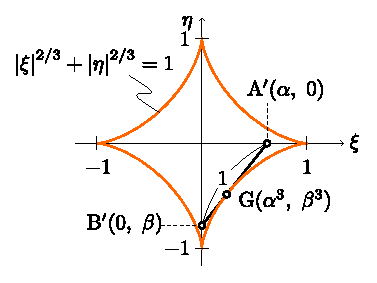
\includegraphics{g107.eps}

The envelope of such a segment is well-known as an \href{https://en.wikipedia.org/wiki/Astroid}{\emph{astroid}}\footnote{Not 
to be confused with {\emph{asteroid}}.}, which is described by the 
equation
$$ \left| \xi \right|^{2/3} + \left| \eta \right|^{2/3} = 1. $$

The image is at the point of tangency $\mathrm{C}$ of the segment 
$\overline{\mathrm{AB}}$ and the envelope of the moving segment, for 
it is the instant point of divergence of the neighboring pencil of rays.
Its corresponding point in the $\xi\eta$-plane is $(K^3, H^3)$.

Thus we can obtain the coordinates of image $(x_{\mathrm{C}}^{}, y_{\mathrm{C}}^{})$ 
from the relation
$$ \left\{ 
\begin{aligned}
	\xi_{\mathrm{C}}^{} &= \dfrac{x_{\mathrm{C}}^{}}{M} = K^3 = \dfrac{\alpha^3}{M^3},\\
	\eta_{\mathrm{C}}^{} &= \dfrac{y_{\mathrm{C}}^{}}{N} = H^3 = \dfrac{\beta^3}{N^3}.
\end{aligned}
\right.$$
That is
$$ \left\{ 
\begin{aligned}
	x_{\mathrm{C}}^{} &= \dfrac{\alpha^3}{M^2},\\
	y_{\mathrm{C}}^{} &= \dfrac{\beta^3}{N^2}=-\dfrac{k^3\alpha^3}{N^2}.
\end{aligned}
\right.$$

Using 
$$\sin\theta_2 = \dfrac{\alpha}{\sqrt{D^2+\alpha^2}},$$
we have
$$k = \dfrac{\sqrt{D^2-(n^2-1)\alpha^2}}{n\alpha},$$
and we can derive the position of the image as parametric functions w.r.t. $\alpha$:
$$ \left\{ 
\begin{aligned}
	x_{\mathrm{C}}^{} &= (n^2-1)\dfrac{\alpha^3}{D^2},\\
	y_{\mathrm{C}}^{} &= -\dfrac{n^2}{D^2}\dfrac{\alpha^3}{n^3\alpha^3}\left\{ D^2-(n^2-1)\alpha^2 \right\}^{3/2}\\
	&=-\dfrac{D}{n}\left\{ 1-(n^2-1)\dfrac{\alpha^2}{D^2} \right\}^{3/2}.
\end{aligned}
\right.$$

\section{POV under water}
If the object is in the air, at height of D above the boundary, and the POV
is under water, the relative index of refraction is $1/n < 1$, and the similar reasoning
leads to the equation
$$ \left| \xi \right|^{2/3} - \left| \eta \right|^{2/3} = -1, $$
with $\xi = \dfrac{x}{W} $ and $\eta = \dfrac{y}{Z}$, where
$W = \dfrac{nD}{\sqrt{1-n^2}}$ and $Z = nD$.

However, I could not find the name for this shape of the curve.  \\

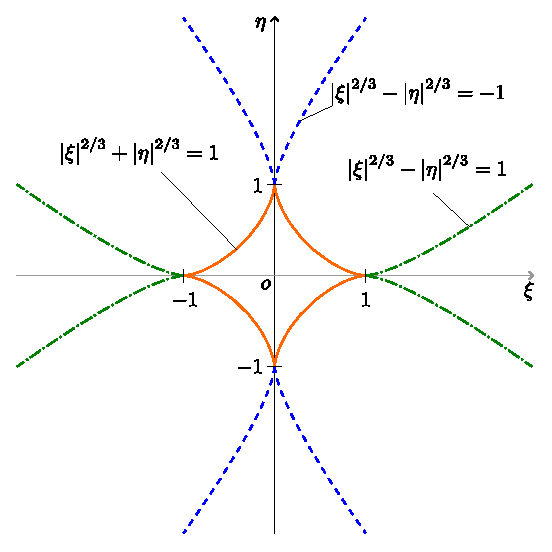
\includegraphics[width=3in]{g254.eps}

If this curve, 
$$ \left| \xi \right|^{2/3} - \left| \eta \right|^{2/3} = \pm1, $$
which has physical significance and is also related to the astroid, does not yet have a name,
how about calling it a \emph{hyperastroid} because it has a relationship with the 
astroid similar to that of a hyperbola to an ellipse?

The astroid is a member of the 
family of curves named \href{https://mathworld.wolfram.com/Astroid.html}{\emph{superellipse}}, which is defined by 
$$ \left| \xi \right|^{r} + \left| \eta \right|^{r} = 1. $$

Asteroid is the case where $r=2/3$. But as far as I know nor is there a name for the 
family of curves in the form
$$ \left| \xi \right|^{r} - \left| \eta \right|^{r} = \pm 1, $$
which could be named \emph{super-hyperbola}, although the repeating cognates may 
bother you\footnote{I might suggest \emph{superbola}.}.

\appendix
\newcommand{\pardiff}[2]{{\frac{\partial #1}{\partial #2}}}
\newcommand{\ilpardiff}[2]{{{\partial #1}/{\partial #2}}}
\section*{Note: Astroid as an envelope}
Let's assume that a point $(K, 0)$ on the x-axis and a point $(0, H)$ on the y-axis in a Cartesian plane move while maintaining a constant distance $a$ between them. Then, $K^2+H^2=a^2$, and the equation of the line containing the line segment at a certain moment can be written as
$$y=-\dfrac{H}{K}(x-K)$$
and using $H=\pm \sqrt{a^2-K^2}$, we have
$$y(x, K) = \mp \dfrac{\sqrt{a^2-K^2}}{K}(x-K)$$
As the value of $K$ changes, the line segment or line connecting the two points changes, and the envelope drawn by it is the locus of stationary points at each moment, that is, the locus of points where $\ilpardiff{y}{K} = 0$. Let's find the $(x, y)$ that satisfy this condition.

$$ \begin{aligned}
	\pardiff{y}{K} &= \pm\left[\left( \dfrac{1}{\sqrt{a^2-K^2}}+\dfrac{\sqrt{a^2-K^2}}{K^2}\right) (x_{0}-K) + \dfrac{\sqrt{a^2-K^2}}{K} \right]\\
	&= \pm \dfrac{(K^2+a^2-K^2)(x_{0}-K)+K(a^2-K^2)}{K^2\sqrt{a^2-K^2}}\\
	&= 0.
\end{aligned}
$$
Therefore the abscissa of the stationary point is $x = K^3/a^2$, and its ordinate is

$$ \begin{aligned}
	y(x, K) &= \mp \dfrac{\sqrt{a^2-K^2}}{K}\left(\dfrac{K^3}{a^2}-K\right)\\
	& = \pm \dfrac{\left( a^2- K^2 \right)^{3/2}}{a^2}\\
	& = \dfrac{H^3}{a^2}
\end{aligned}
$$
Therefore, the coordinate $(x, y)$ of the stationary points satisfies the equation
$$ \left|\dfrac{x}{a}\right|^{2/3} + \left|\dfrac{y}{a}\right|^{2/3} = 1. $$
$\blacksquare$

\end{document}

